\chapter{Vers une génération de rapports automatique à partir d’imagerie avec MyoQuant}
\section{Contexte}
Les outils présentés précédemment ont pour vocation de traiter et d'explorer les comptes-rendus de biopsie textuels. Permettant ainsi une approche rétrospective de l'ensemble des patients connu à ce jour. Cependant il est intéressant d'explorer aussi comment l'analyse d'images par \gls{ia} peut permettre de générer automatiquement ces comptes-rendus de biopsie. Cette approche permettrait un grain de précision et de temps dans l'évaluation des biopsies. Tout d'abord un gain de temps car une approche par \gls{ia} permettrait de traiter  plusieurs biopsies de grande taille de manière automatique, libérant ainsi le temps utilisé pour l'évaluation des coupes histologiques. Ensuite un gain de précision car l'évaluation des biopsies par un expert humain est en général qualitative. La description de phénotype se limite généralement à des adjectifs de quantité tels que "peu", "moyen" ou "beaucoup". Grâce à une approche de comptage par \gls{ia}, il est alors possible d'obtenir la quantité précise de fibres présentant un noyau centralisé par exemple et ainsi de pouvoir établir des seuils pour une analyse plus approfondie.

\gls{myoquant}, l'outil présenté dans ce chapitre, est une suite de méthodes pour quantifier différents marqueurs pathologiques dans les biopsies de \gls{mc}. \gls{myoquant} intègre soit des méthodes algorithmiques simples basées sur des modèles d'\gls{ia} généralistes en histologie comme CellPose (\cite{stringer_cellpose_2021}) et Stardist (\cite{weigert_star-convex_2020}), soit des méthodes basées sur des modèles \gls{ia} développés à partir de nos données. Actuellement, \gls{myoquant} est capable de quantifier des marqueurs pathologiques dans trois des cinq colorations réalisées en routine lors du diagnostic des \gls{mc}: la centralisation des noyaux à la coloration \gls{he}, un déséquilibre dans le ratio des fibres de type 1 et 2 à la coloration ATPase et une répartition anormales des mitochondries dans les fibres musculaires à la coloration \gls{sdh}. Dans ce chapitre nous allons voir comment ont été implémentées ces solutions de quantification automatique et des exemples d'application.

\begin{figure}[htbp]
 \centering
 
\includegraphics[width=0.66\textwidth]{figures/myoquant_logo.png}
 \caption[Logo MyoQuant]{Logo de MyoQuant}
 \label{fig:myoquant_logo}
\end{figure}

\section{Analyse de la position des noyaux cellulaires}
Dans un premier temps, nous nous sommes intéressés à l'analyse de la position des noyaux cellulaires dans les fibres musculaire. Dans un muscle sain, les noyaux sont en général en périphérie des fibres, chez les patients atteints de \gls{mc} et particulièrement dans les \gls{cnm}, les noyaux peuvent être internalisés voir centralisés. Par exemple, dans la figure \ref{fig:he_example}, on observe un nombre important de fibres ayant un noyau cellulaire internalisé. Nous avons alors développé une méthode pour compter automatiquement le nombre de fibres présentant un noyau internalisé.
\begin{figure}[htbp]
 \centering
 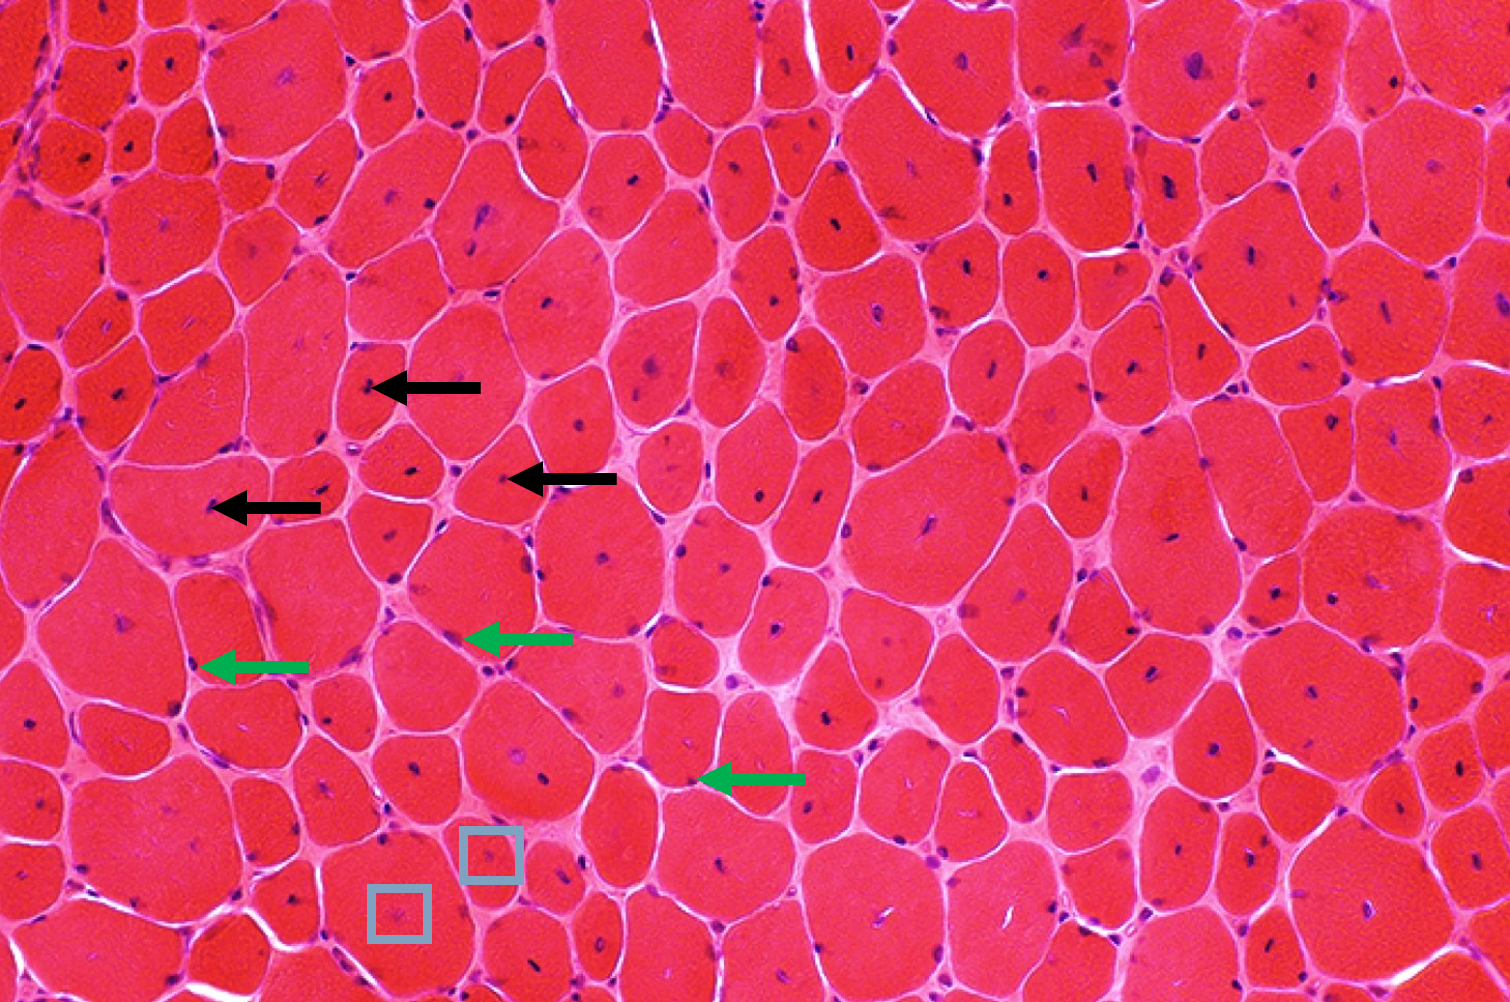
\includegraphics[width=0.8\textwidth]{figures/he_example.jpg}
 \caption[Exemple de biopsie musculaire à la coloration HE]{Exemple de biopsie musculaire de CNM à la coloration HE dans laquelle on observe des fibres avec des noyaux centralisés.}
 \label{fig:he_example}
\end{figure}

\subsection{Algorithme de quantification}
Pour réaliser cette quantification, la première étape consiste à segmenter, c'est-à-dire obtenir la position de toutes les fibres musculaires et les noyaux de la coupe. Pour cela nous avons utilisés deux modèles d'\gls{ia} généralistes développés spécifique pour l'analyse de coupes histologiques: Cellpose et Stardist. Cellpose nous a permis de segmenter les fibres musculaires, tandis que Stardist nous a permis de segmenter les noyaux cellulaires. La figure \ref{fig:he_seg} présente les résultat de la segmentation de la biopsie présentée en figure \ref{fig:he_example}. On observe que globalement toutes les fibres musculaires sont bien segmentées, cependant concernant les noyaux cellulaires, certains sont trop peu colorés pour être reconnus par le modèle. C'est notamment le cas pour quelques noyaux centraux sur la gauche de la biopsie. Ce qui sera problématique lors de l'analyse des noyaux, car ils ne seront pas considérés.
\begin{figure}[htbp]
 \centering
 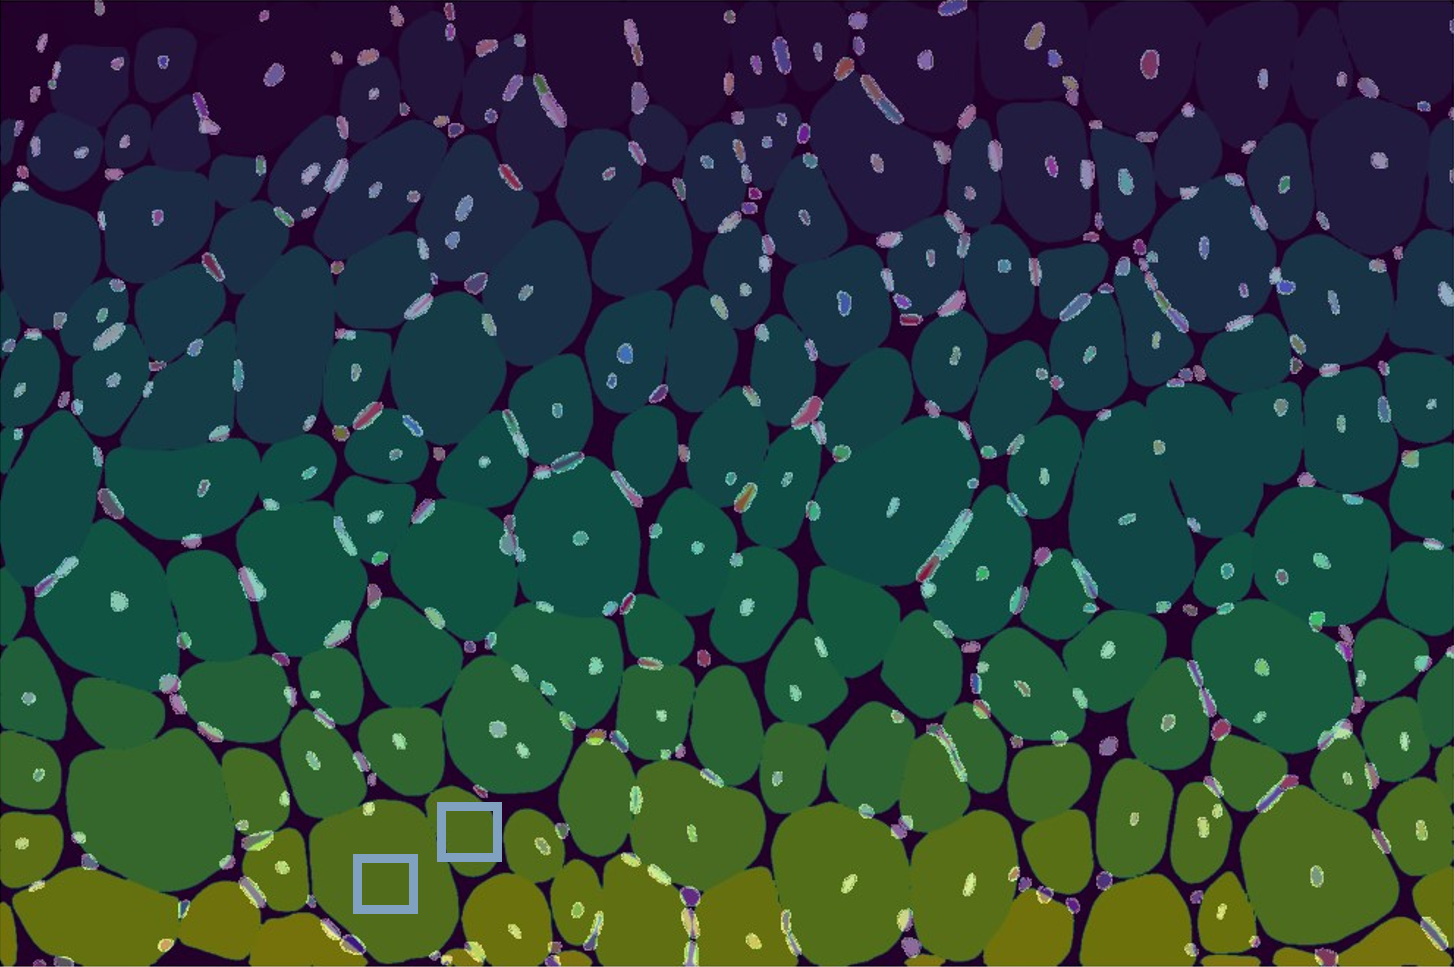
\includegraphics[width=0.8\textwidth]{figures/he_seg.png}
 \caption[Exemple de segmentation de biopsie par Cellpose et Stardist]{Exemple de segmentation des fibres musculaires et des noyaux cellulaires par Cellpose et Stardist}
 \label{fig:he_seg}
\end{figure}

Une fois avoir obtenu la position de chaque fibre et noyaux, nous évaluons la position de chaque noyaux, fibre par fibre. Cette évaluation repose sur le calcul de ce que l'on appelle un score d'excentricité. Ce score est calculé selon la formule suivante:

\(\text{Score d'excentricité} = \frac{\text{Dist. centre fibre et noyau}}{\text{Dist. centre fibre et membrane}}\)

Dans cette formule la notation "Dist. centre fibre et noyau" représente la distance en pixels entre le centroïde de la fibre musculaire et centroïde du noyau considéré. Et la notation "Dist. centre fibre et membrane" représente la distance entre le centroïde de la fibre musculaire et la membrane cellulaire selon une droite passant par le noyau d'intérêt. La figure \ref{fig:he_single_nuc}  présente la classification des noyaux d'une fibre musculaire unique. Quatre noyaux ont été détectés dans cette fibre dont trois ont un score d'excentricité supérieur à 0,9 et un inférieur à 0,1. En fixant un seuil de façon empirique à 0,75, on considère alors que cette fibre musculaire possède un noyau internalisé.
\begin{figure}[htbp]
 \centering
 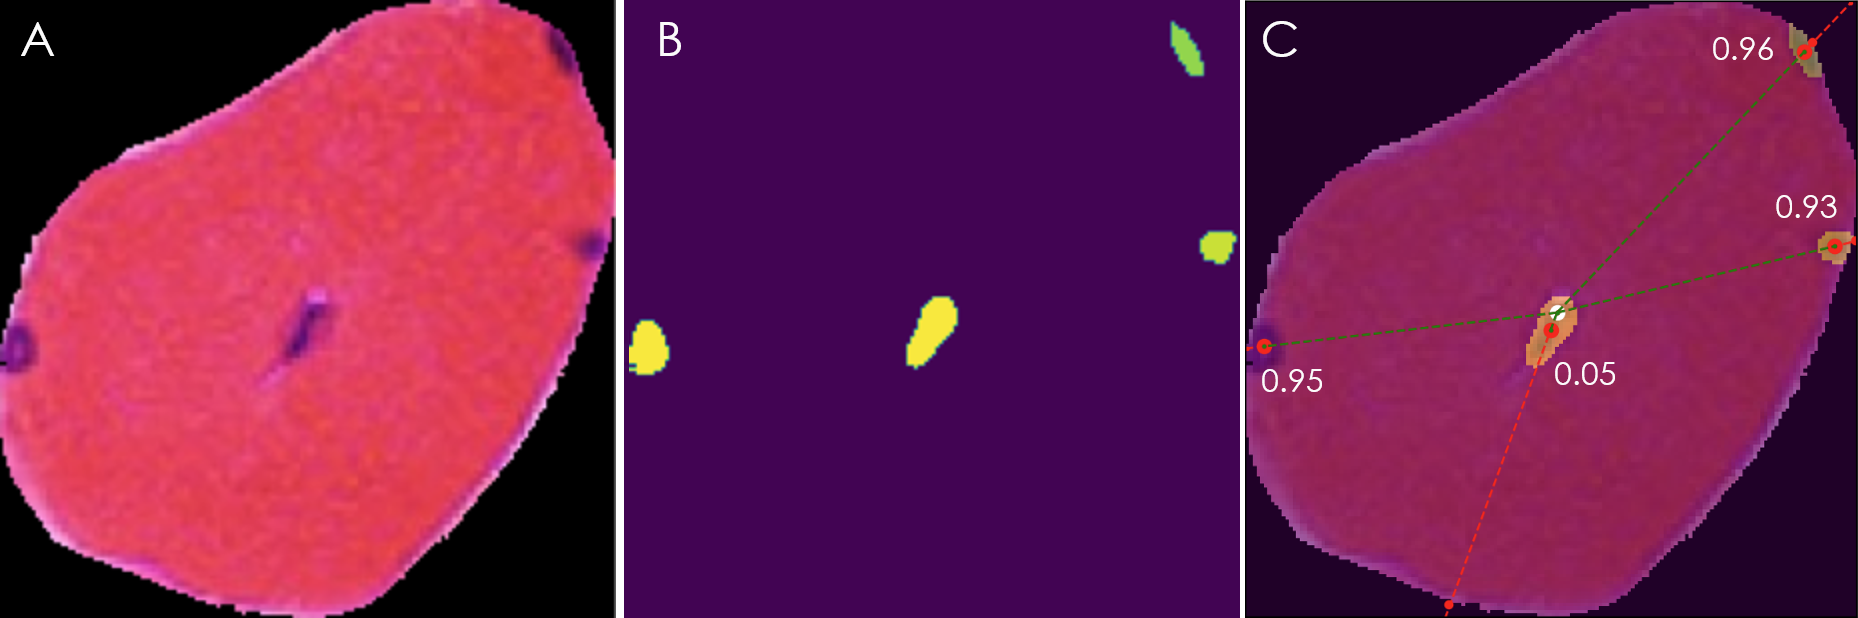
\includegraphics[width=1\textwidth]{figures/he_single_nuc.png}
 \caption[Exemple de classification de la position des noyaux]{Exemple de classification de la position des noyaux cellulaire d'une fibre musculaire. \textbf{(A)} La fibre musculaire seule,\textbf{ (B)} masque de segmentation des 4 noyaux pour cette fibre,\textbf{ (C)} schéma de la classification des noyaux avec le score d'excentricité de chaque noyau représentant le ratio de distance: centre de la fibre - noyau vs centre de la fibre - membrane cellulaire.}
 \label{fig:he_single_nuc}
\end{figure}
En comparant l'ensemble des noyaux de chaque fibre à un seuil (ici fixé à 0,75) on peut alors quantifier le nombre de fibres musculaires ayant au moins un ou plusieurs noyaux internalisés. Par exemple pour l'image présentée en figure \ref{fig:he_example}, la figure \ref{fig:he_paint} présente les résultats de cette classification. Sur cette coupe histologique, on obtient un total de 74 fibres (soit 42\% des fibres) avec au moins un noyau internalisé.
\begin{figure}[htbp]
 \centering
 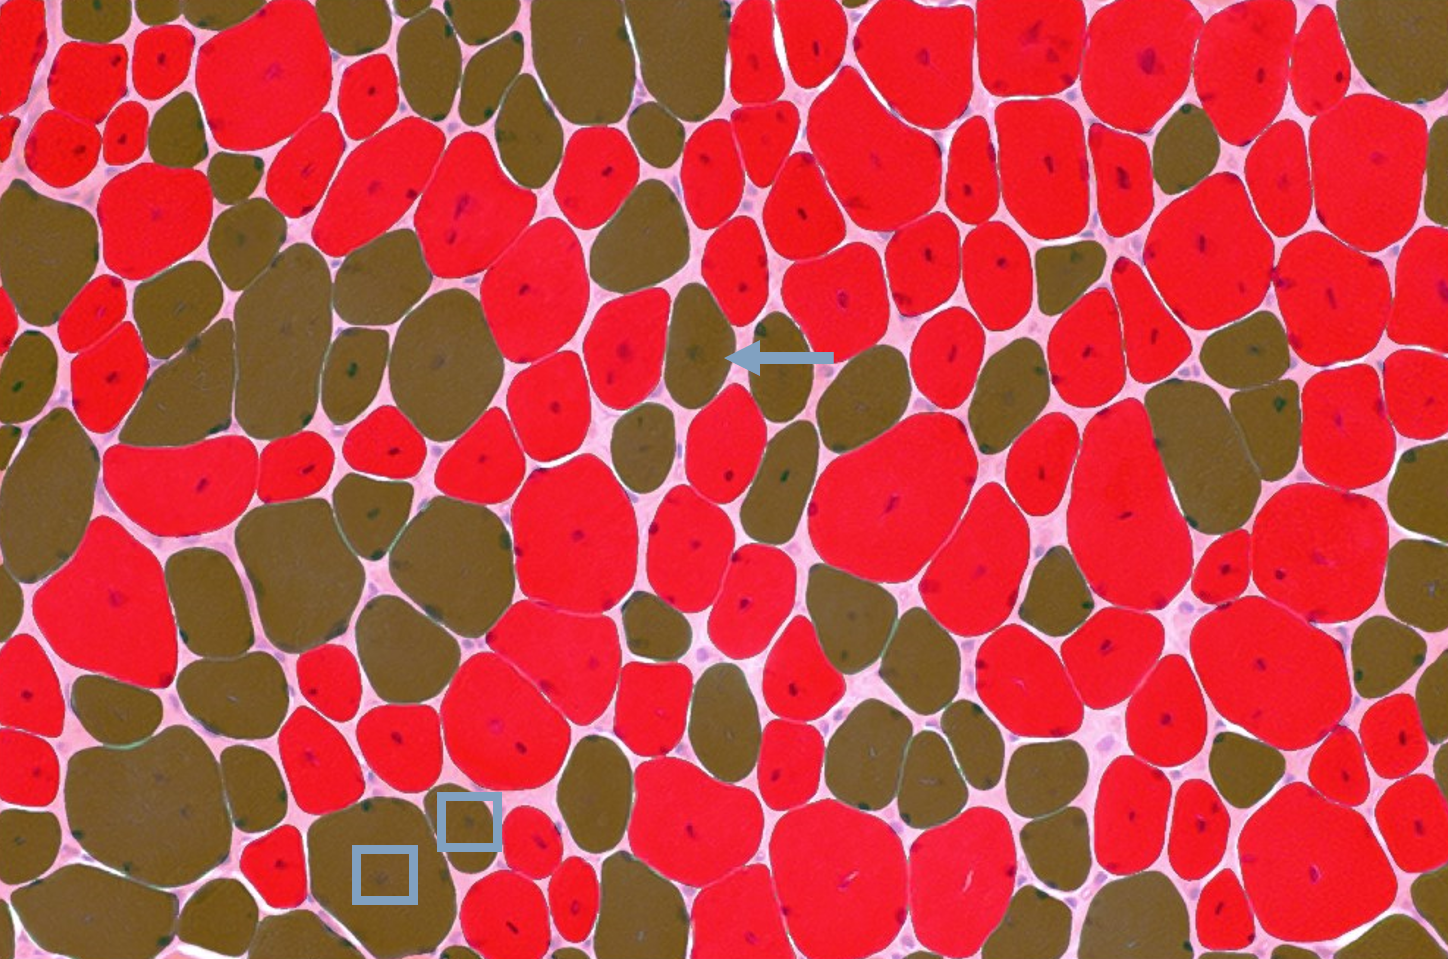
\includegraphics[width=0.8\textwidth]{figures/he_paint.png}
 \caption[Exemple de classification de biopsie musculaire à la coloration HE]{Exemple de classification de biopsie musculaire à la coloration HE. Colorées en vert les fibres sans noyau internalisé, et en rouge les fibres avec au moins un noyau internalisé (score d'excentricité inférieur à 0.75)}
 \label{fig:he_paint}
\end{figure}

\subsection{Exemple d'application: quantification de la régénération musculaire }
La présence de noyaux centralisés dans les fibres musculaires est un marqueur pathologique dans les biopsies de \gls{mc}. Cependant cette centralisation peut aussi être synonyme de régénération musculaire chez les individus sains. Ainsi, la quantification du nombre de noyaux centralisés est donc aussi un moyen de quantifier la régénération musculaire dans une coupe histologique. Dans le cadre d'une collaboration avec l'\gls{igbmc} et spécifiquement avec l'équipe Biologie moléculaire et cellulaire des cancers du sein du Dr. Tomasetto, nous avons utilisé \gls{myoquant} pour évaluer la quantité de régénération musculaire chez des souris traitées avec un drogue induisant le processus régénération. Ces images d'histologie sont des images à fluorescence (et non à la coloration \gls{he}) avec un fluorochrome pour la membrane cellulaire et un fluorochrome pour les noyaux cellulaire. L'algorithme de \gls{myoquant} est directement compatible avec les images à fluorescence et fonctionne de la même façon que pour les images à coloration\gls{he}
\begin{figure}[htbp]
 \centering
 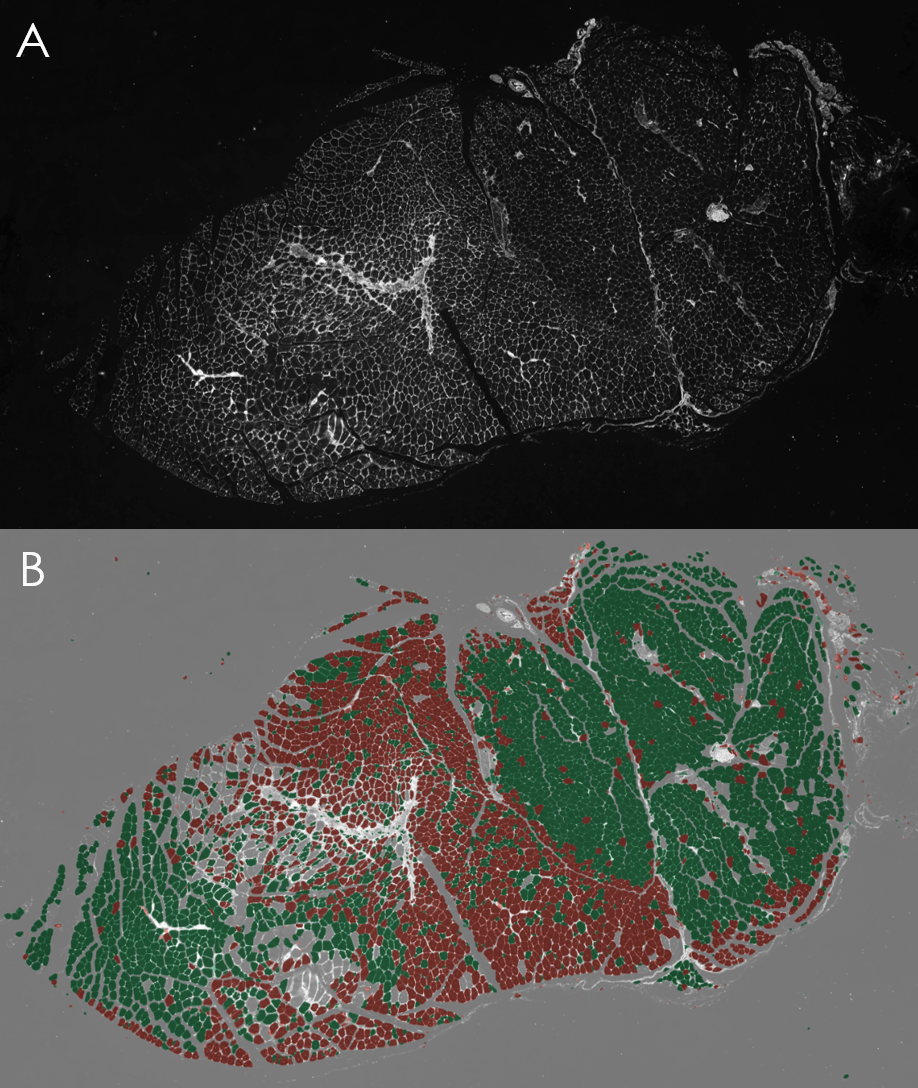
\includegraphics[width=0.8\textwidth]{figures/fluo_nuc.png}
 \caption[Exemple de classification de biopsie musculaire pour la régénération musculaire]{Exemple de classification de biopsie musculaire pour la régénération musculaire. Colorées en vert les fibres sans noyau internalisé (fibres normales), en rouge les fibres avec au moins un noyau internalisé (en régénération)}
 \label{fig:fluo_paint}
\end{figure}

La figure \ref{fig:fluo_paint} présente un exemple de coupe complète de biopsie musculaire de souris avec le masque de quantification associé généré par \gls{myoquant}. Sur cette image, il y a 6078 fibres musculaires détectées, dont 2285 (environ 35\%) sont en régénération. Le tableau \ref{tab:myoquant_fluo_time} présente le temps de calcul nécessaire pour chaque étape de la quantification pour la coupe \ref{fig:fluo_paint} et le tableau \ref{tab:myoquant_fluo_results} présente les résultats de cette quantification. On observe ici que pour traiter une coupe complète sur une machine sans matériel spécifique (sans \gls{gpu}) il a nécessité environ 1 heure de calcul, dont la majorité a été utilisée par Cellpose pour segmenter les fibres musculaires. Cependant cette vitesse peut être largement améliorée d'un facteur 5 par l'utilisation de matériel spécifique aux calculs \gls{ia} (\gls{gpu}), passant de 3782 secondes pour Cellpose à 652. Pour une image contenant 6078 fibres et 23 628 noyaux, cela représente environ 1.6 fibre traitée par seconde. Cette quantification a mis en évidence que 37\% des fibres présentaient un noyau internalisé et donc sont en régénération.
\begin{table}[htbp]
\centering
\caption{Temps de calcul pour l'analyse des noyaux d'une coupe complète (6078 fibres, 12000 x 9600 pixels)}
\label{tab:myoquant_fluo_time}
\begin{tabularx}{\textwidth}{|l|c|c|X|}
\hline
\textbf{Étape} & \textbf{Temps sur GPU} & \textbf{Temps sur CPU (s)} & \textbf{Fibres par seconde (sur CPU)} \\
\hline
Cellpose & 652 & 3 782 & 1.6 \\
\hline
StarDist & \textit{mémoire insuffisante} & 21 & 29 \\
\hline
Classification des noyaux & 68 & 68 & 89 \\
\hline
\textbf{Total} & \textbf{>720} & \textbf{3 871} & \textbf{1.57} \\
\hline
\end{tabularx}
\end{table}

\begin{table}[htbp]
\centering
\caption{Résultats de quantification des noyaux d'une coupe complète (6078 fibres, 12000 x 9600 pixels)}
\label{tab:myoquant_fluo_results}
\begin{tabular}{|l|c|c|}
\hline
\textbf{Type} & \textbf{Valeur} & \textbf{Proportion (\%)} \\
\hline
N° Fibres & 6 078 & 100 \\
\hline
N° Fibres avec 1+ noyau internalisé & 2 264 & 37 \\
\hline
\hline
N° Noyaux & 23 628 & 100 \\
\hline
N° Noyaux internalisés & 3 933 & 16 \\
\hline
N° Noyaux périphériques & 17 918 & 76 \\
\hline
N° Noyaux non-classés (hors fibres) & 1 777 & 8 \\
\hline
\end{tabular}
\end{table}
Le tableau \ref{fig:fluo_compil} présente l'ensemble des quantifications opérées dans les différentes conditions de traitement et de génotype (au total 35 \gls{wsi} analysées). On observe qu'après traitement avec la \textit{Cardiotoxin}, une drogue induisant la régénération musculaire, une proportion significativement supérieur de fibres ayant un noyaux internalisé par rapport aux coupes contrôle. Ces résultats confirment que \gls{myoquant} est bien capable d'évaluer de façon robuste la présence de noyaux internalisés, un marqueur de la régénération musculaire.

\begin{figure}[htbp]
 \centering
 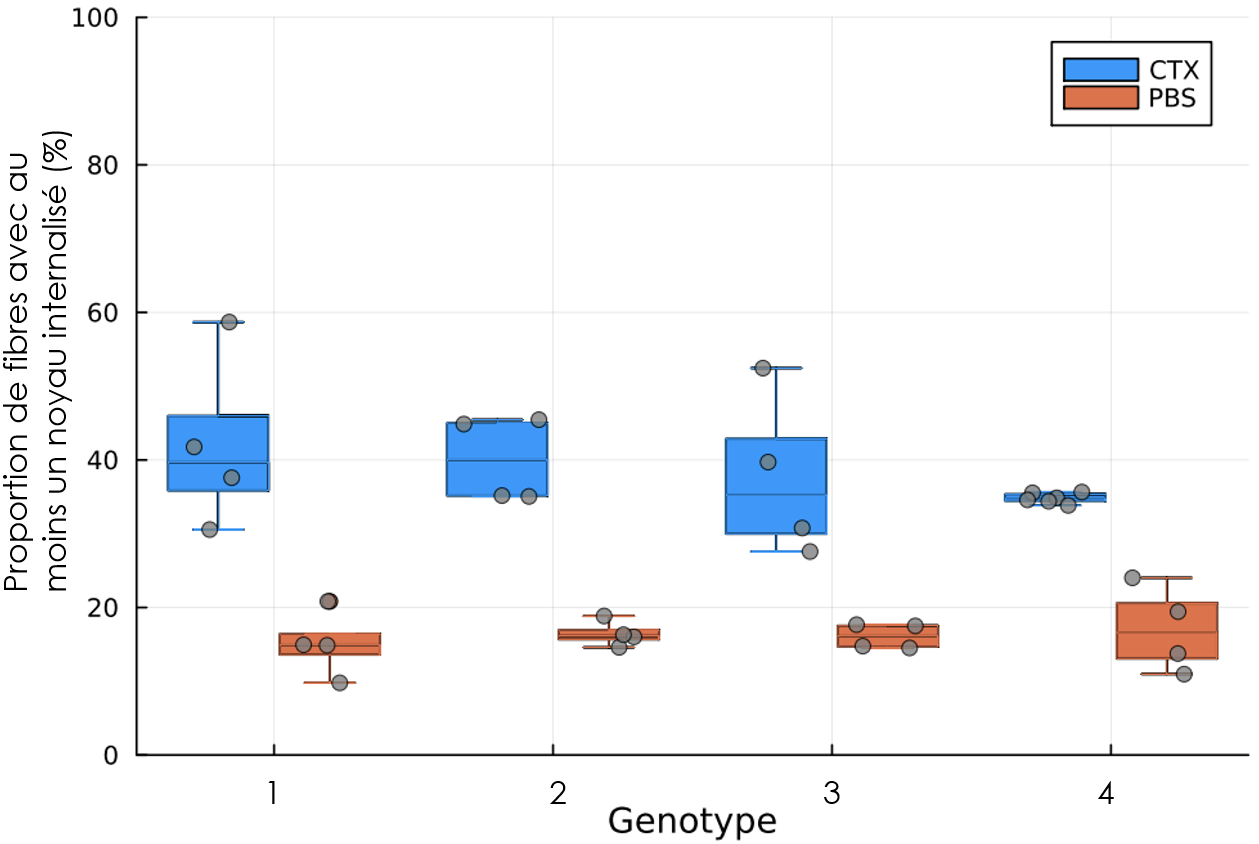
\includegraphics[width=0.8\textwidth]{figures/fluo_compil.png}
 \caption[Résultat de la quantification de la régénération musculaire]{Résultat de la quantification de la régénération musculaire chez des souris pour 4 génotypes différents traités (bleu) ou non (orange) avec une drogue induisant la régénération musculaire}
 \label{fig:fluo_compil}
\end{figure}

\section{Ratio de fibre de type 1 et 2: classification basée sur l'intensité de coloration}

Dans un second temps, nous nous sommes intéressés à l'analyse du ratio des différents types de fibres musculaires dans les biopsies. Dans certaines \gls{mc}, l'équilibre entre fibres de type 1 et type 2 peut être modifié avec une prédominance des fibres de type 1. Les différents types de fibres musculaires sont colorées différentiellement (différence d'intensité) à la coloration ATPase. A un pH 4.3, les fibres de type 1 sont sombres et les fibres de type 2 sont pâles, et inversement au pH 9.4. La figure \ref{fig:atp_example} représente une biopsie musculaire colorée à l'ATPase pH 9.4. On observe la présence de deux populations de fibres à intensité de coloration distinctes. Nous avons alors développé une méthode pour compter automatiquement le nombre de fibres de chaque type.
\begin{figure}[htbp]
 \centering
 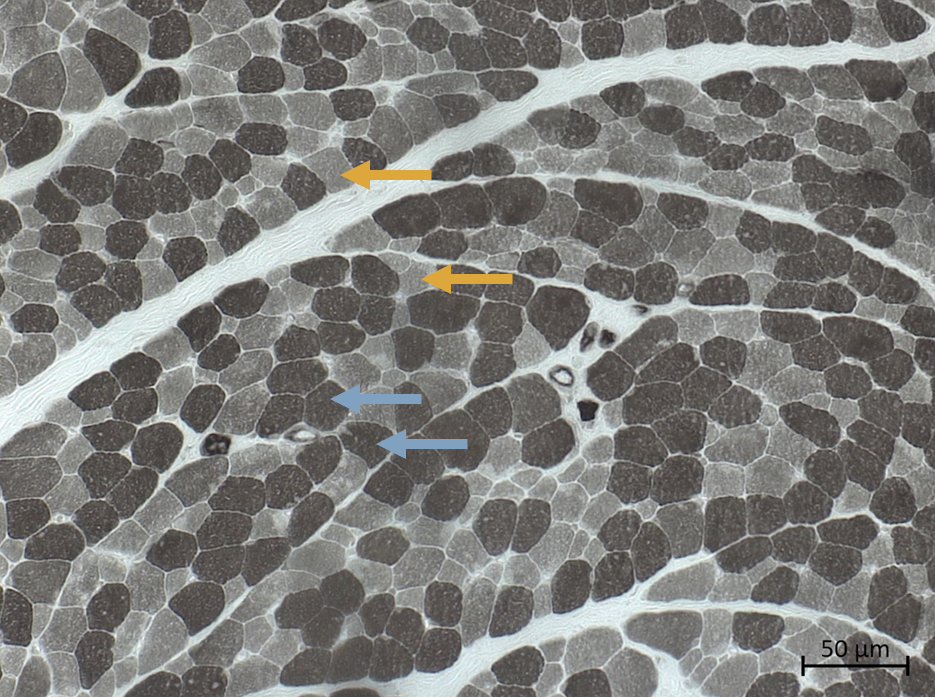
\includegraphics[width=0.8\textwidth]{figures/atp_example.png}
 \caption[Exemple de biopsie musculaire à la coloration ATPase pH 9.4]{Exemple de biopsie musculaire à la coloration ATPase pH 9.4 qui permet de différencier les fibres de type 1 aux fibres de type 2.}
 \label{fig:atp_example}
\end{figure}
\subsection{Algorithme de quantification}
Pour réaliser cette quantification, la première étape consiste à segmenter, c'est-à-dire obtenir la position de toutes les fibres musculaires. Comme précédemment, nous avons utilisés Cellpose afin segmenter les fibres musculaires. Ensuite pour chaque fibre nous avons extrait l'intensité moyenne de la fibre et avons réalisé un histogramme. La figure \ref{fig:atp_density} présente l'histogramme issu de l'analyse de l'image d'exemple pour la coloration ATPase pH 9.4 (\ref{fig:atp_example}). Le but de la procédure est de déterminer automatiquement les pics présents dans l'histogramme et de trouver les minimums locaux entre les pics pour fixer un ou plusieurs seuil d'intensité. Pour cela, à partir des valeurs de cet histogramme, une courbe de densité est créée (par méthode de \gls{kde}). Puis à partir de cette courbe de densité, une méthode de mélange Gaussien est utilisée pour déterminer la position des pics dans la courbe de densité. Finalement, le seuil est déterminé en trouvant le minimum local de la courbe de densité entre les deux pics obtenu par mélange Gaussien.
\begin{figure}[htbp]
 \centering
 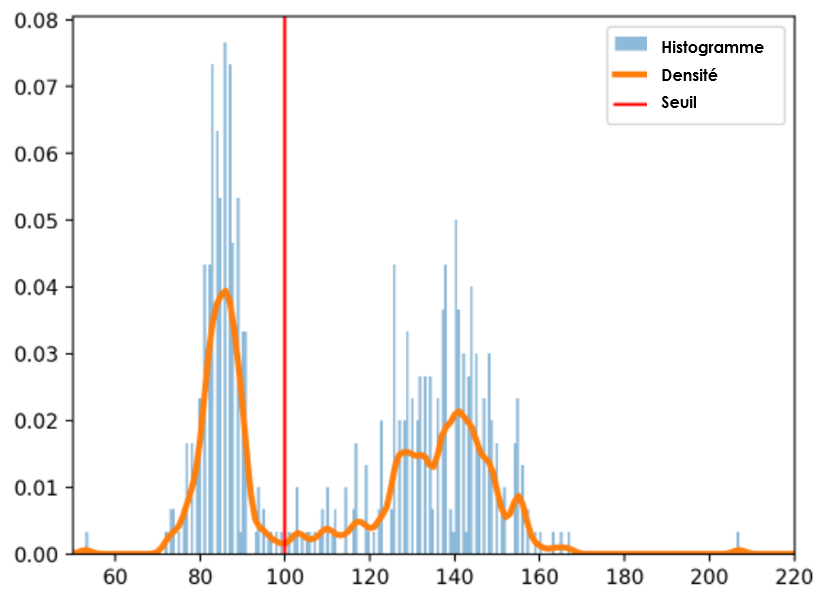
\includegraphics[width=0.8\textwidth]{figures/density_plot.png}
 \caption[Exemple d'histogramme et courbe de densité biopsie ATPase]{Exemple d'histogramme et courbe de densité biopsie ATPase}
 \label{fig:atp_density}
\end{figure}

A partir de ce seuil, il est alors possible de classer les fibres musculaire en deux catégories: celles avec une intensité moyenne inférieure au seuil et celles avec une intensité moyenne supérieure. La figure \ref{fig:apt_paint} présente les résultats de la quantification automatique des fibres de l'image présentée en exemple précédemment. Sur cette image, on a pu quantifier au total la présence de 496 fibres, dont 269 (54\%) fibres de type 1 et 227 (46\%) fibres de type 2. 
\begin{figure}[htbp]
 \centering
 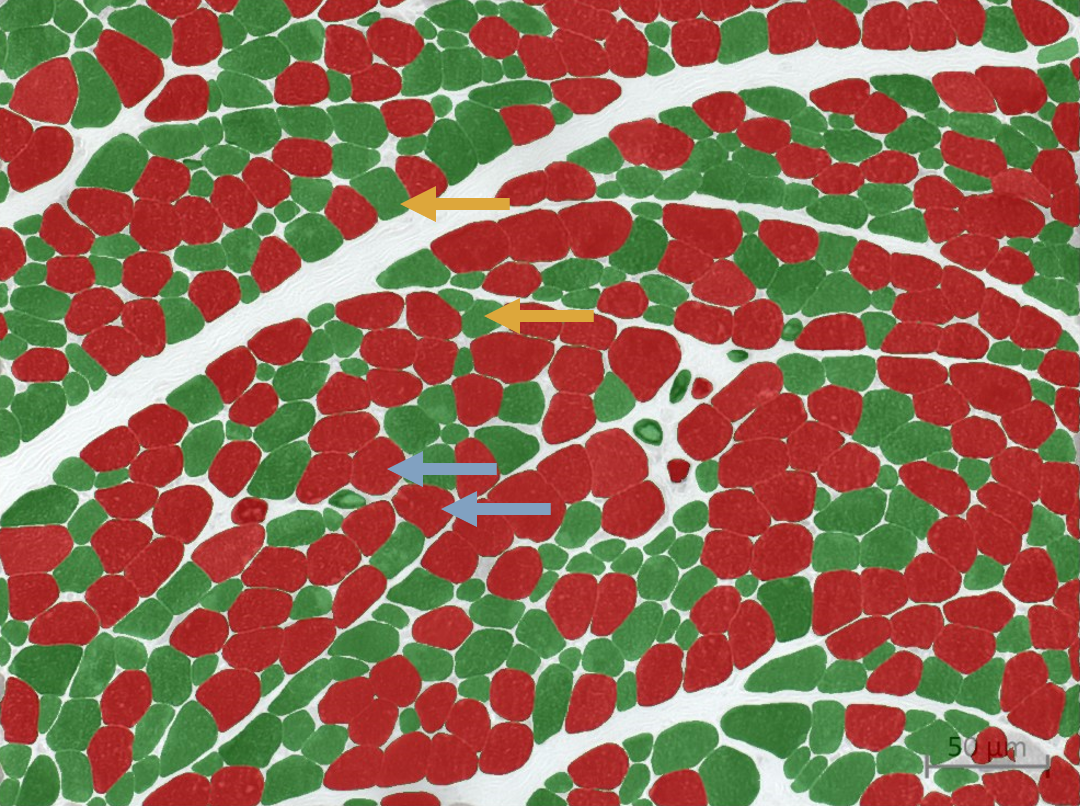
\includegraphics[width=0.8\textwidth]{figures/atp_paint.png}
 \caption[Exemple de classification de biopsie musculaire à la coloration ATPase pH 9.4]{Exemple de classification de biopsie musculaire à la coloration ATPase pH 9.4. Colorées en rouge les fibres ayant une intensité inférieure au seuil (type 2) en vert supérieure au seuil (type 1)}
 \label{fig:apt_paint}
\end{figure}

\subsection{Exemple d'application: classification d'une coupe complète avec trois types de fibres}
La coloration ATPase peut révéler plus de deux types de fibres musculaires. En effet les fibres de type 2 ont plusieurs sous-type visualisables dans certaines conditions de coloration. Dans cet exemple, nous avons utilisé la méthode de classification développée pour détecter trois types de fibres. L'algorithme présenté dans cette section est capable d'établir autant de seuils automatiquement que spécifiés par l'utilisateur.. La figure \ref{fig:atp_paint_wsi} présente les résultats de classification d'une \gls{wsi} de biopsie musculaire colorée à l'ATP pH 4.6. Sur cette coupe on observe trois populations de fibres: des fibres pâles (fibres de type 2A), des fibres intermédiaires (fibres de type 2B) et de petites fibres très sombres localisées en haut de la coupe (fibres de type 1). La méthode de quantification a alors pu définir deux seuils pour séparer ces trois classes. 
\begin{figure}[htbp]
 \centering
 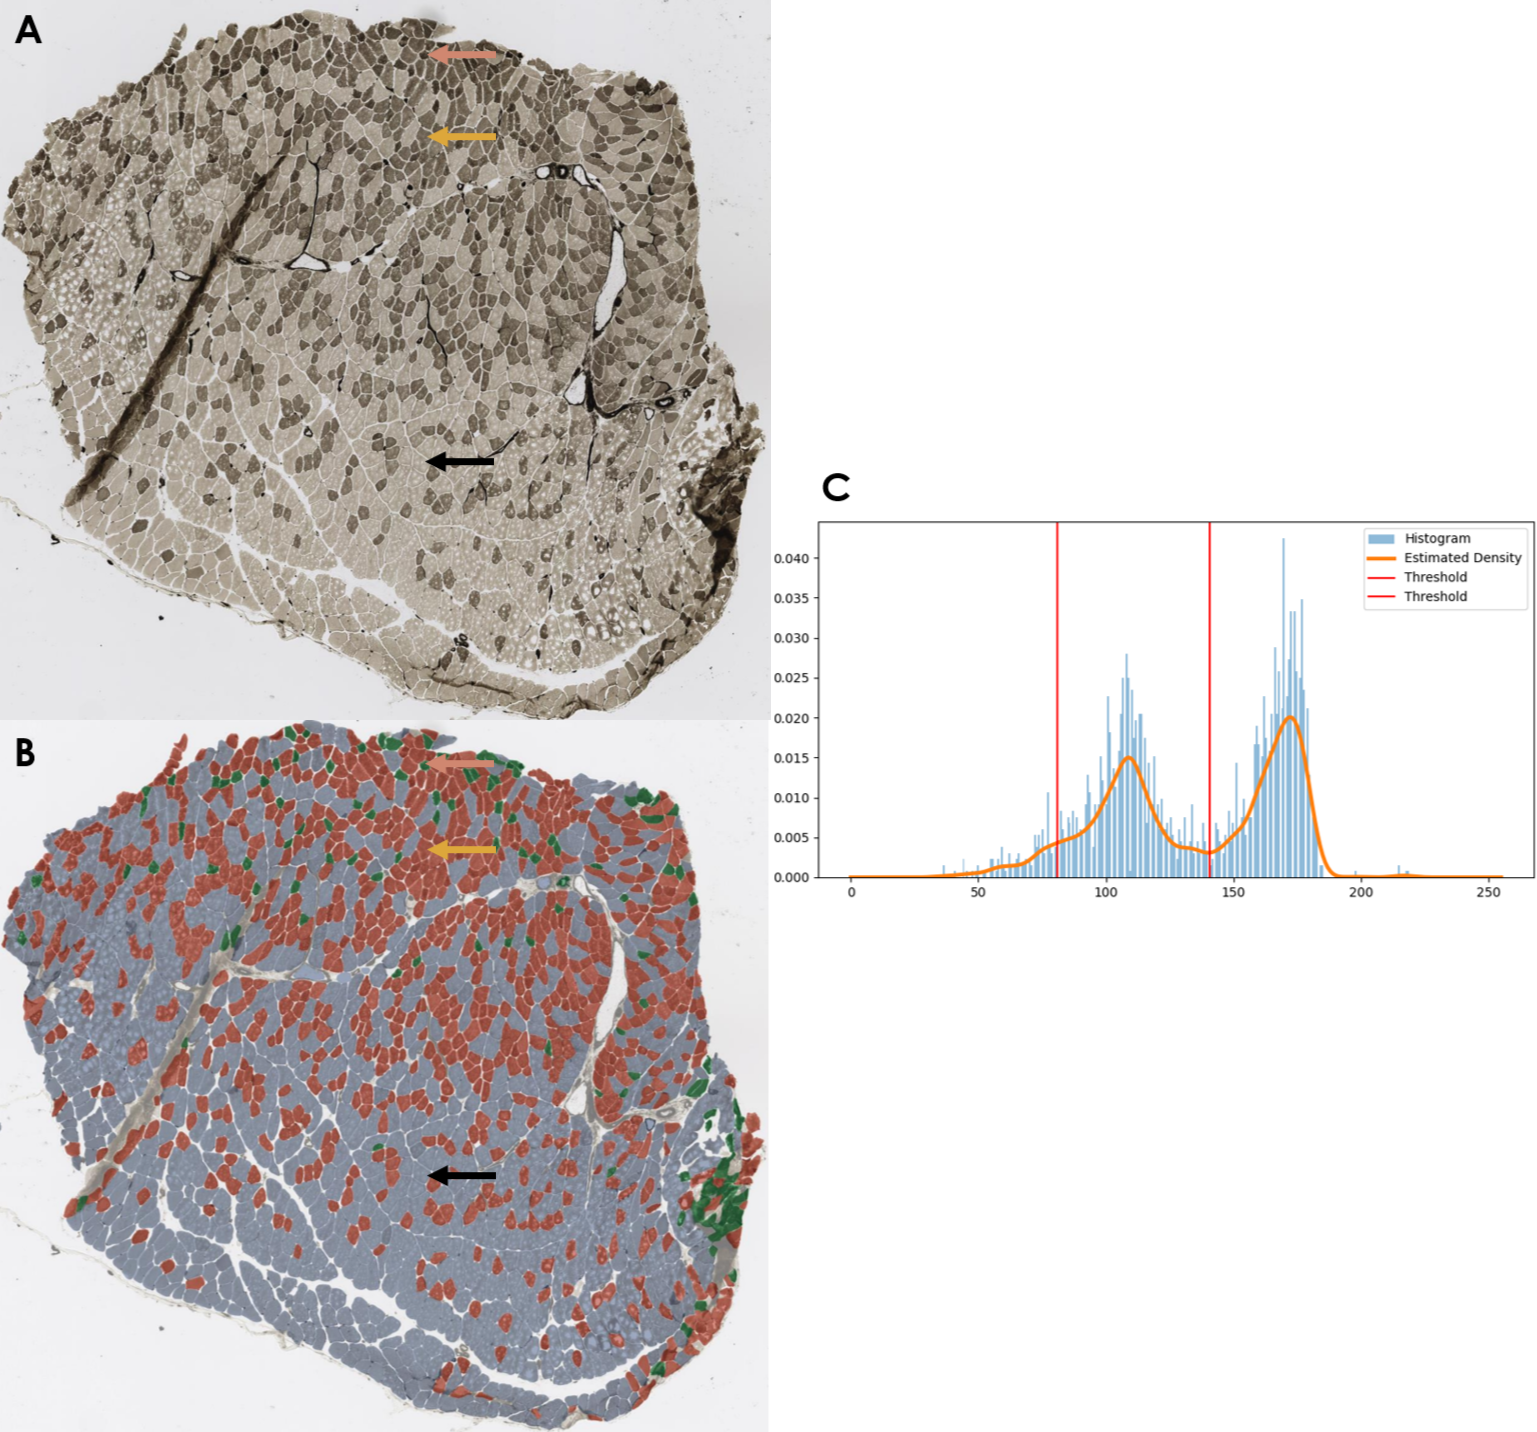
\includegraphics[width=1\textwidth]{figures/atp_wsi.png}
 \caption[Exemple de classification de biopsie musculaire colorée à l'ATPase]{Exemple de classification de biopsie musculaire colorée à l'ATPase en 3 classes: en bleu les fibres de type 2A, en rouge les fibres de type 2B et en vert les fibre de type 1.}
 \label{fig:atp_paint_wsi}
\end{figure}

Les résultats de cette classification sont référencés dans le tableau \ref{tab:atp_wsi_resultstable} , le temps de calcul et la vitesse de classification sont disponibles dans le tableau \ref{tab:atp_wsi_timetable}. Au total, 1840 fibres ont été classifiées en 131 secondes (soit 14 fibres par seconde). Il y a une majorité de fibres de type 2A (894, 49\%), de fibres de type de 2B (829, 45\%) et une faible proportion de petites fibres de type 1 (117, 6\%). Les résultats de cette quantification sont visuellement satisfaisants, bien qu'une partie de la biopsie en bas a droite, est repliée sur elle-même et donc apparaît avec une intensité de coloration forte. Cette zone a donc été considérée à tort comme des fibres de type 1. Ces résultats mettent en évidence le besoin de biopsies avec une préparation de qualité pour obtenir des résultats robustes lors de la quantification automatique.

\begin{table}[htbp]
\centering
\caption{Temps de calcul pour l'analyse des types de fibres d'une coupe complète (1840 fibres, 6000 x 5600 pixels)}
\label{tab:atp_wsi_timetable}
\begin{tabular}{|l|c|c|}
\hline
\textbf{Étape} & \textbf{Temps sur GPU} & \textbf{Fibre par seconde (sur GPU)} \\
\hline
Cellpose & 113 & 16 \\
\hline
Classification des fibres & 18 & 102 \\
\hline
\textbf{Total} & \textbf{131} & \textbf{14} \\
\hline
\end{tabular}
\end{table}
\begin{table}[htbp]
\centering
\caption{Résultats de quantification des types de fibre d'une coupe complète (1840 fibres, 6000 x 5600 pixels)}
\label{tab:atp_wsi_resultstable}
\begin{tabular}{|l|c|c|}
\hline
\textbf{Type} & \textbf{Valeur} & \textbf{Proportion (\%)} \\
\hline
Fibre type 2A & 894 & 49 \\
\hline
Fibre type 2B & 829 & 45 \\
\hline
Fibre type 1 & 117 & 6 \\
\hline
\end{tabular}
\end{table}


\section{Répartition des mitochondries: classification par IA}
Enfin, nous nous sommes intéressés à l'analyse de la répartition des mitochondries dans les fibres musculaires. Cette répartition peut être anormale dans certaines \gls{mc}. Cette répartition se visualise grâce à la coloration \gls{sdh}, révélant l'activité oxydative des fibres musculaires et donc la position des mitochondries. La figure \ref{fig:sdh_example} présente un exemple de biopsie de muscle de souris modèle de myopathie congénitale à la coloration \gls{sdh}. On observe deux types de fibres, des fibres "normales" ayant une répartition homogène en coloration et des fibres "anormales" ayant une agglutination de coloration au centre de la fibre (notamment sur la gauche de la coupe), représentant des agrégats mitochondriaux pathologiques. Nous avons alors développé une méthode capable de détecter et de compter les fibres ayant une répartition mitochondriale anormale, en développant notre propre modèle d'\gls{ia}.

\begin{figure}[htbp]
 \centering
 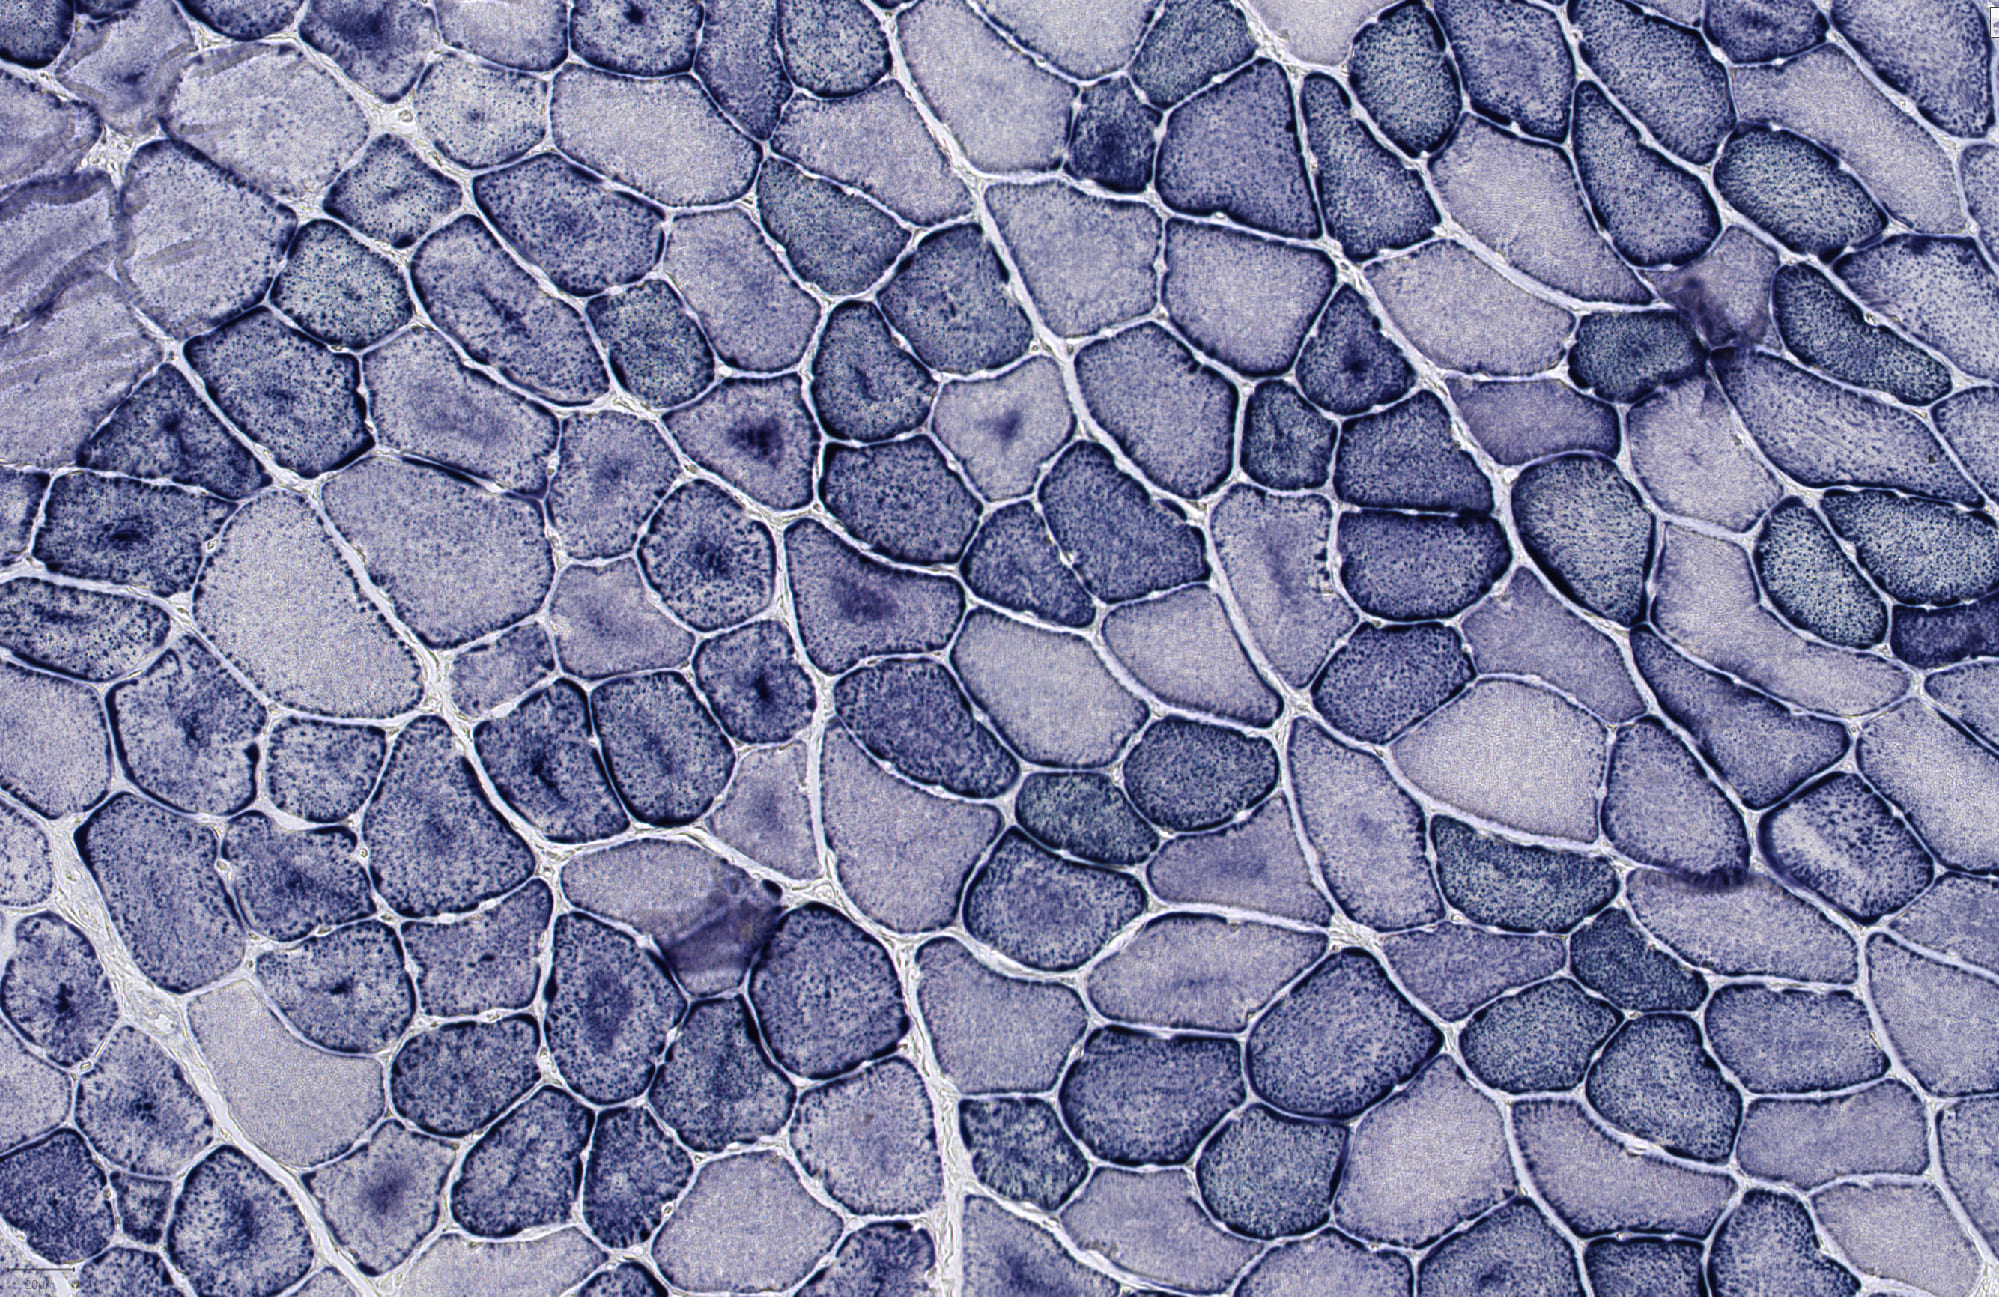
\includegraphics[width=0.8\textwidth]{figures/sdh_example.jpg}
 \caption[Exemple de biopsie musculaire à la coloration SDH]{Exemple de biopsie de muscle de souris modèle de CNM à la coloration SDH}
 \label{fig:sdh_example}
\end{figure}
\subsection{Jeu de données d'image de muscle de souris et annotations}
Pour constituer le jeu de données nécessaire à l'entraînement de cette \gls{ia} nous avons utilisés 18 \gls{wsi} de biopsies musculaires de souris, dont une souris saine (\textit{wild-type}) et 17 \gls{wsi} de souris modèles de \gls{cnm} (10 \textit{Bin1-KO} et 7 \textit{Dnm2S619L}). Ces 18 \gls{wsi} représentent un total de 16 787 fibres musculaires (tableau \ref{tab:sdh_fiber_count}). Chacune de ces fibres musculaires a été isolée et extraite de la coupe grâce à Cellpose puis a été annotée à la main en 2 catégories: fibre saine ou anormale, par l'expert ayant généré les images (Quentin Giraud et Charlotte Gineste). Au total, les 12 730 fibres saines et 4 057 fibres annotées comme anormales ont été séparées équitablement en trois jeux de données: 72\% pour le jeu d'entraînement de l'\gls{ia}, 8\% pour le jeu de validation lors de l'entraînement, et 20\% pour le jeu de test des performances de l'\gls{ia}. Ce jeu de données à été mis à disposition de la communauté scientifique de façon \textit{open-source} sur la plateforme \textit{Hugging-Face} à l'adresse: \href{https://huggingface.co/datasets/corentinm7/MyoQuant-SDH-Data}{https://huggingface.co/datasets/corentinm7/MyoQuant-SDH-Data}.

\begin{table}[htbp]
\centering
\caption{Répartition des fibres pour le jeu d'entraînement du modèle SDH}
\label{tab:sdh_fiber_count}
\begin{tabular}{|c|c|c|c|c|}
\hline
 & \textbf{Entraînement} (72\%) & \textbf{Validation} (8\%) & \textbf{Test} (20\%) & \textbf{Total} \\
\hline
\textbf{Saine} & 9 165 & 1 019 & 2 546 & 12 730 (76\%) \\
\hline
\textbf{Anormale} & 2 920 & 325 & 812 & 4 057 (24\%) \\
\hline
\hline
\textbf{Total} & 12 085 & 1 344 & 3 358 & 16 787 \\
\hline
\end{tabular}
\end{table}


\subsection{Architecture, entraînement et performance du modèle IA}
A partir de ce jeu de données, nous avons entraîné un modèle de \gls{cnn}. Nous avons sélectionné l'architecture réseau de neurones profonds \textit{Resnet50} pré-entraînée sur \textit{ImageNet}. L'architecture \textit{Resnet50} est une architecture à l'état de l'art pour la classification d'images et le pré-entraînement sur \textit{ImageNet} permet d'obtenir de meilleures performance et une convergence du modèle accélérée. Pour limiter le sur-apprentissage, nous avons appliqué des techniques d'augmentation de données lors de l'apprentissage par variation de luminosité, contraste, rotation aléatoire, zoom, translation et retournement. De plus, nous avons utilisé une méthode d'arrêt prématuré pour arrêter l'entraînement lorsque que les performances sur le jeu de validation ne se sont pas améliorées lors des 10 dernières époques. Enfin chaque fibre musculaire unique a été re-dimensionnée à une taille de 256x256 pixels, car le réseau de neurones impose une taille d'image constante.
\begin{figure}[htbp]
 \centering
 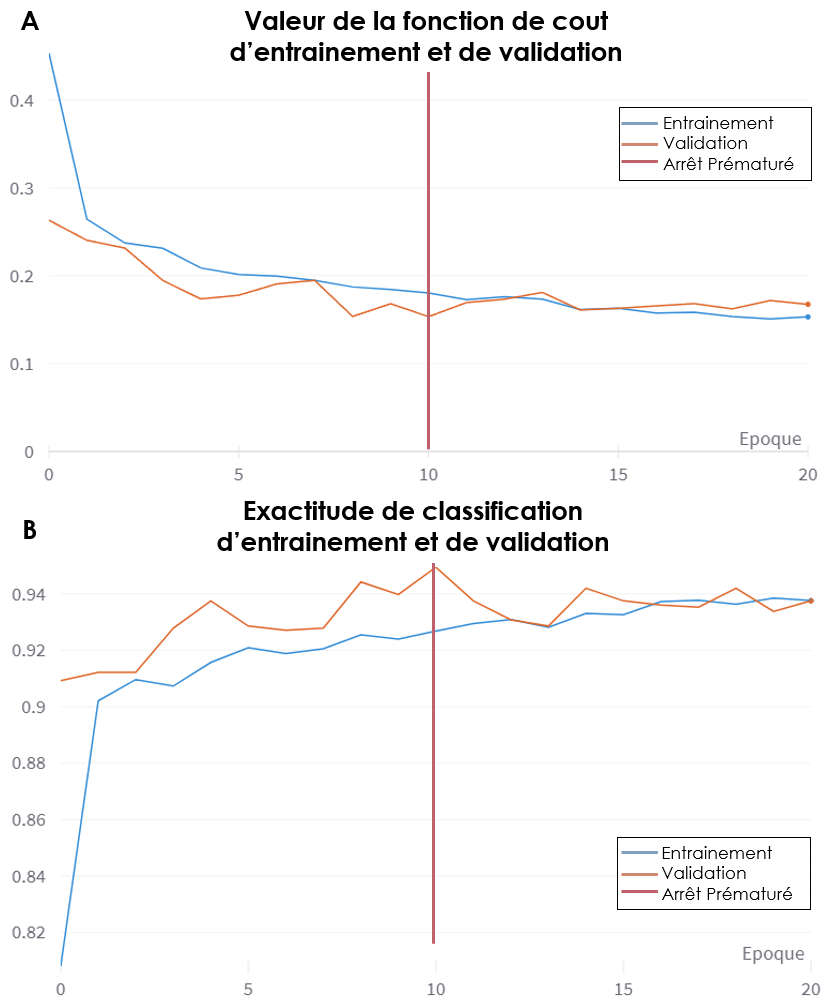
\includegraphics[width=1\textwidth]{figures/training_sdh.png}
 \caption[Courbe d'apprentissage du modèle SDH]{Courbe d'apprentissage du modèle SDH. En haut la courbe d'erreur, en bas la courbe d'exactitude de classification pour le jeu d'entraînement (bleu) et le jeu de validation (orange). La barre verticale rouge indique le modèle final sélectionné par arrêt prématuré.}
 \label{fig:sdh_train}
\end{figure}

La figure \ref{fig:sdh_train} présente les courbes d'apprentissage du modèle \gls{sdh}. Que ce soit en terme de mesure de l'erreur du modèle (\textit{loss}) ou d'exactitude de classification, on observe qu'après 10 époques (12 minutes d'entraînement), les performances sont maximales pour le jeu de validation et ne s'améliorent plus sur les 10 époques suivantes. Ceci indique qu'après 10 époques, l'apprentissage donne lieu à un sur-apprentissage du jeu d'entraînement. C'est pourquoi grâce à l'arrêt prématuré, nous avons sélectionné le modèle dans l'état après 10 époques comme modèle optimal sans sur-apprentissage.

Après la phase d'apprentissage, pour mesurer les performances du modèle nous avons utilisé le jeu de test composé de 3358 images qui n'ont pas été utilisées pour l'entraînement. En comparant les prédictions du modèle sur les images de test à leur annotation par les experts, nous avons obtenu une exactitude de classification de 93,2\% et une exactitude pondérée de 91.7\%. Autrement dit, le modèle est capable de reproduire l'annotation des deux experts avec une exactitude de 93,2\%.

L'ensemble des métriques mesurées lors de l'entraînement sont disponibles de façon open-source à l'adresse: \href{https://wandb.ai/lambda-science/myoquant-sdh}{https://wandb.ai/lambda-science/myoquant-sdh}, le modèle ainsi que le code-source utilisés pour réaliser cet entraînement de manière reproductible sont aussi disponibles sur la plateforme \textit{HuggingFace} à l'adresse: \href{https://huggingface.co/corentinm7/MyoQuant-SDH-Model}{https://huggingface.co/corentinm7/MyoQuant-SDH-Model}.

\subsection{Exemple d'application}
Grâce au modèle développé, il est maintenant possible de classer des fibres individuelles pour détecter les anomalies de répartition mitochondriale. Ainsi pour analyser une image complète, on utilise d'abord Cellpose pour segmenter et isoler chaque fibre musculaire de l'image puis le modèle que nous avons développé pour prédire la classe de la fibre. Par exemple pour l'image de biopsie présentée ci-dessus (\ref{fig:sdh_example}), le résultat de classification est présenté en figure \ref{fig:sdh_paint}. Au total sur 162 fibres détectées, 86 (53\%) sont classées comme ayant une répartition mitochondriale anormale et 76 (46\%) ont une répartition normale. On observe que ce sont bien les fibres ayant une agglutination de coloration au centre de la fibre (agrégats de mitochondries, sur la gauche de la coupe) qui sont classées comme anormales, confirmant le bon fonctionnement du modèle.

\begin{figure}[htbp]
 \centering
 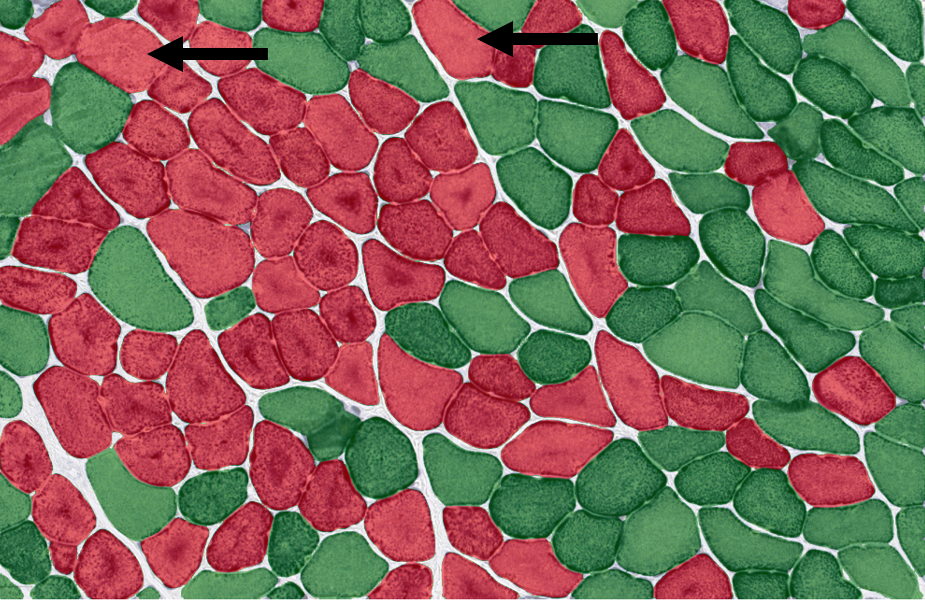
\includegraphics[width=0.8\textwidth]{figures/sdh_paint.png}
 \caption[Exemple de classification de biopsie musculaire de souris à la coloration SDH]{Exemple de classification de biopsie musculaire de souris à la coloration SDH. Colorées en rouge les fibres ayant répartition mitochondriale anormale, en vert une répartition normale}
 \label{fig:sdh_paint}
\end{figure}
\begin{figure}[htbp]
 \centering
 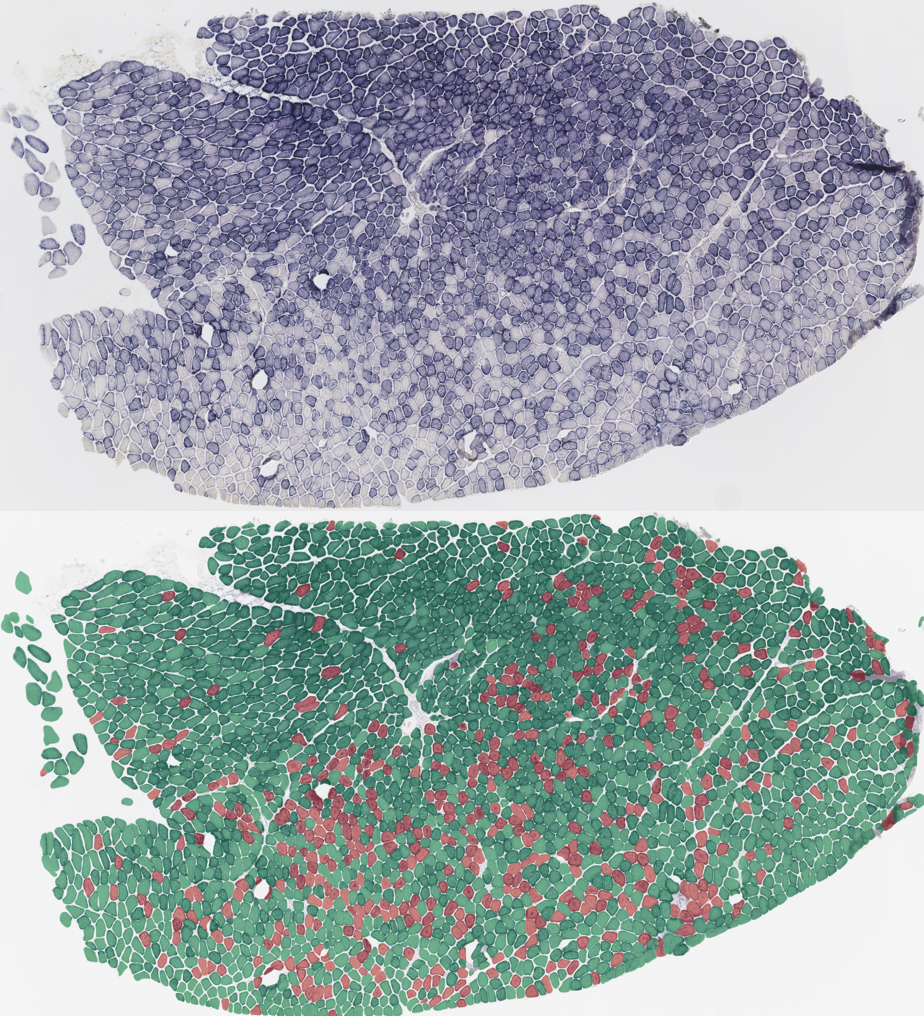
\includegraphics[width=0.8\textwidth]{figures/wsi_sdh.png}
 \caption[Exemple de classification de coupe complète biopsie musculaire de souris à la coloration SDH]{Exemple de classification de coupe complète biopsie musculaire de souris à la coloration SDH. Colorées en rouge les fibres ayant répartition mitochondriale anormale, en vert une répartition normale}
 \label{fig:sdh_wsi_paint}
\end{figure}

Il est aussi possible de classer des \gls{wsi} de biopsie de muscle complet colorées au \gls{sdh}. Par exemple la figure \ref{fig:sdh_wsi_paint} présente les résultats de classification d'une coupe complète comptant 2 869 fibres musculaires. En terme de ressources de calcul, l'étape limitante reste le modèle Cellpose qui, pour cette image, requiert trop de mémoire pour fonctionner sur notre matériel (\gls{gpu}). Ainsi sur CPU, nous avons eu besoin d'environ 40 minutes pour quantifier la coupe, dont la majorité du temps à servis à Cellpose,  ce qui représente une vitesse d'environ 1 fibre par seconde. Au final sur la coupe présentée, 2371 fibres sont classées comme saines (83\%) et 498 sont classées comme anormales (17\%).

\begin{table}[htbp]
\centering
\caption{Temps de calcul pour l'analyse des fibre d'une coupe complète SDH (2 869 fibres, 11200 x 6300 pixels)}
\label{tab:sdh_wsi_timetable}
\begin{tabularx}{\textwidth}{|l|c|c|X|}
\hline
\textbf{Étape} & \textbf{Temps sur GPU} & \textbf{Temps sur CPU} & \textbf{Fibre par seconde (sur CPU)} \\
\hline
Cellpose & \textit{Mémoire insuffisante} & 2 407 & 1,2 \\
\hline
Classification des fibres & 70 & 66 & 43 \\
\hline
\textbf{Total} & \textbf{>70} & \textbf{2473} & \textbf{1,15} \\
\hline
\end{tabularx}
\end{table}
\begin{table}[htbp]
\centering
\caption{Résultats de quantification des  fibre d'une coupe complète SDH (2 869 fibres, 11200 x 6300 pixels)}
\label{tab:sdh_wsi_resultstable}
\begin{tabular}{|l|c|c|}
\hline
\textbf{Type} & \textbf{Valeur} & \textbf{Proportion (\%)} \\
\hline
Fibres saines & 2371 & 83 \\
\hline
Fibres anormales & 498 & 17 \\
\hline
\end{tabular}
\end{table}


\subsection{Exploration du modèle}
Une fois le modèle entraîné, nous avons voulu explorer le modèle grâce à différentes techniques de visualisation pour nous assurer que ses capacités de classification sont bien réelles et ne sont pas dues à un biais lors de l'apprentissage.

\subsubsection{Explicabilité de la classification}
Afin de vérifier sur quels critères la classification des fibres est réalisée, nous avons utilisé la méthode Grad-Cam (\textit{Gradient-weighted Class Activation Mapping}, \cite{selvaraju_grad-cam_2020}). Cette méthode permet de générer une carte thermique des images pour visualiser les régions importantes pour la classification selon le modèle. Cette carte thermique est réalisée en utilisant les gradients de la sortie par rapport aux cartes de \textit{features} des couches convolutives pour chaque classe, puis une moyenne pondérée est calculée.

\begin{figure}[htbp]
 \centering
 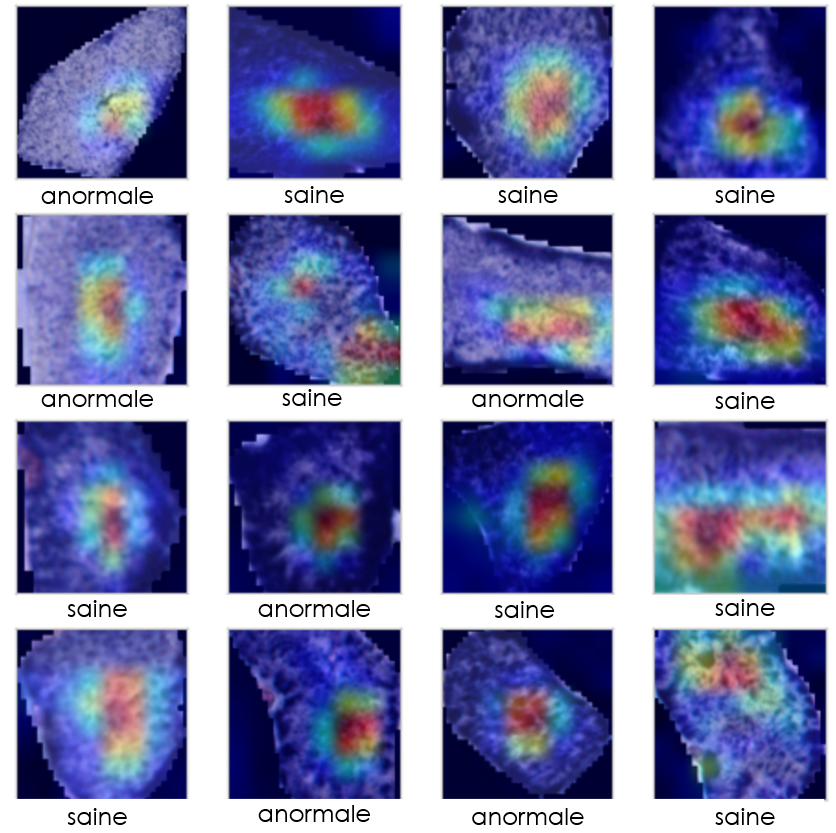
\includegraphics[width=0.8\textwidth]{figures/sdh_gradcam.png}
 \caption[Visualisation par méthode \textit{Grad-Cam} du modèle SDH]{Visualisation par méthode  \textit{Grad-Cam} de la classification de 16 fibres prises au hasard du jeu de test par modèle SDH. Superposition de l'image originale re-dimensionnée et de la carte thermique générée}
 \label{fig:gradcam_sdh}
\end{figure}
La figure \ref{fig:gradcam_sdh} présente les résultats de cette méthode de visualisation sur 16 fibres musculaires uniques prise au hasard dans le jeu de test. On observe sur cette figure que la zone déterminante pour la classification des fibres selon le modèle est le centre de la fibre musculaire. Cette observation est cohérente car nous avons observé que dans la majorité des cas, une fibre est dite anormale lorsqu'elle présente une agglutination de coloration au centre de la fibre (agrégats de mitochondries centralisés). Cette méthode confirme donc que le modèle porte son attention globalement sur la même zone que l'expert lors de la classification manuelle. 

\subsubsection{\textit{Embedding} des images et réduction de dimensionalité} 
Pour rappel la notion d'\textit{embedding} correspond  à la transformation d'une donnée en un vecteur numérique de grande taille. Dans \gls{nlmyo} nous avons utilisé des technique d'\textit{embedding} sur des données textuelles. Ici, nous avons réalisé un \textit{embedding} de nos images non pas pour faire de la classification mais pour appliquer des techniques de réduction de dimensionalité (comme une PCA) pour visualiser si notre modèle est bien capable des faire une différence net entre les deux classes.
Pour cela nous avons utilisé notre modèle \gls{sdh} et avons retiré la dernière couche de neuronnes servant à la classification. Ainsi la sortie du modèle correspond à la sortie de la dernière couche convolutive, c'est-à-dire à un vecteur de taille (1, 2048) correspondant aux caractéristiques importantes de l'image extraites par le modèle pour la classification.  En réalisant cette opération pour l'ensemble des images nous obtenons une matrice (16 787, 2048) sur laquelle nous appliquons une méthode de réduction de dimensionalité (nommée UMAP (\cite{mcinnes_umap_2020})), donnant ainsi une matrice (16 787, 2) visualisable facilement.
\begin{figure}[htbp]
 \centering
 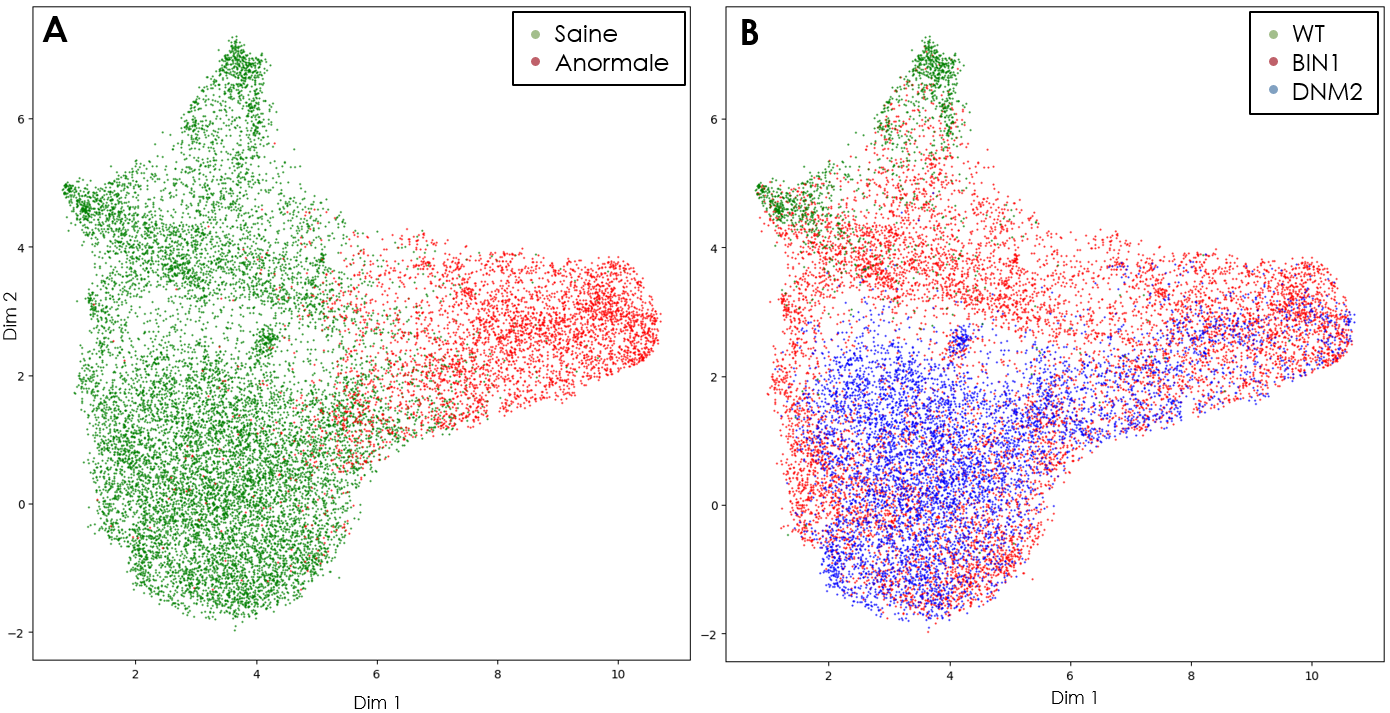
\includegraphics[width=1\textwidth]{figures/umap_sdh.png}
 \caption[Visualisation de l'\textit{embedding} du modèle SDH]{Visualisation de l'\textit{embedding} du modèle SDH des 16 787 images de fibres musculaires après réduction de dimensionalité par UMAP. A gauche, les fibres sont colorées par label, à droite elles sont colorées par modèle de souris}
 \label{fig:umap_sdh}
\end{figure}

Ainsi la figure \ref{fig:umap_sdh} présente la visualisation obtenu après \textit{embedding} et réduction de dimensionalité des 16 787 images du jeu de données. Chaque point représente une image du jeu de données, colorée selon son label (annotation) ou sa provenance (modèle de souris). Globalement on observe que sur le premier (et donc le plus important) axe de variance (en abscisse), le modèle extrait des informations permettant de faire la différence entre les fibres saines et anormales. En effet les deux classes de fibres sont bien séparés avec cependant la présence d'un continuum entre les deux groupes indiquant la présence de fibres avec des profils complexes, "entre deux". Le second axe de variance (en ordonné) indique que le modèle extrait aussi des informations permettant de d'établir le provenance de la fibre, c'est à dire de quel modèle de souris elle est issue. En effet on voit un cluster de fibres venant de souris \textit{wild-type} assez compact en haut de la figure, puis deux clusters à la fois superposés et séparés de fibres provenant de souris modèle \textit{BIN1} et \textit{DNM2}. L'ensemble des ces résultats confirment que notre modèle extrait et base sa classification des fibres sur les caractéristiques intrinsèques des fibres saines ou anormales et non pas sur des biais extérieurs.

\subsubsection{Identification des erreurs d'annotation par le modèle}
Lors de la phase de test, le modèle a obtenu une exactitude de classification de 93.2\%, il existe donc une marge de progression pour le modèle. Les 6.8\% d'erreur peuvent être expliqué par plusieurs raisons. La première est que le modèle n'est peut-être pas assez complexe pour capturer l'ensemble des critères de classification des images et donc a des difficultés pour certains cas complexes. Cependant nous utilisons un modèle à l'état de l'art \textit{Resnet50} avec plus de 25 millions de paramètres, ce qui devrait être suffisant pour cette tache de classification. Un seconde raison pourrait être la présence de bruit ou d'erreurs dans le jeu de données de base. Nous avons alors voulu explorer comment nous pouvions grâce au modèle entraîné, explorer le jeu de donnés initial pour potentiellement trouver des erreurs d'annotation.

La figure \ref{fig:identify_errors} résume la démarche utilisée pour identifier des erreurs dans le jeu de données. A partir de la prédiction de la classe des 16 787 images, nous avons filtré pour ne garder que les images où le label (annotation par l'expert) était discordant avec la prédiction du modèle ET où le modèle avait un fort niveau de confiance dans la prédiction (>85\%). Au total cela représente 228 images soit 1.66\% du jeu de donnée de base.
\begin{figure}[htbp]
 \centering
 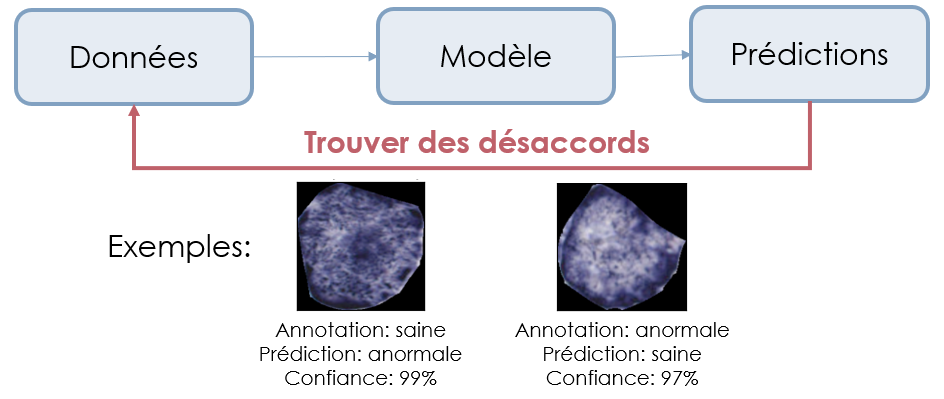
\includegraphics[width=1\textwidth]{figures/identify_errors.png}
 \caption[Méthode d'identification des potentielles erreurs d'annotation]{Méthode d'identification des potentielles erreurs d'annotation}
 \label{fig:identify_errors}
\end{figure}

La figure \ref{fig:list_errors} présente huit exemples pris au hasard parmi les 228 images ayant une prédiction discordante avec l'annotation et un haut niveau de confiance du modèle. On observe par exemple pour la première et la dernière image, qu'elle ont été annotées comme saines et prédites comme anormales par le modèle. En regardant l'image de la fibre, on observe une tache centrale caractéristique de fibres ayant une répartition mitochondriale anormale. Ceci laisse donc penser qu'il y a eu une erreur d'annotation pour ces deux fibres, considérée à tort comme saines. De même pour la seconde image, annotées comme anormale mais prédite comme saine, on observe la présence d'un marquage homogène sans agglutination caractéristique du marquage au centre, il n'y a donc visiblement pas de raison pour la classer comme anormale.

Ces résultats montrent que le modèle est capable après entraînement d'identifier des erreurs humaines lors de l'évaluation des fibres. Ces erreurs d'annotation peuvent être dues à des inattentions ou des erreurs de clic lors du travail manuel et répétitif d'annotation des  16 787 images par les experts. La détection de potentielles erreurs par le modèle et leur ré-annotation pourraient permettre d'améliorer le jeu de données utilisé pour l'entraînement du modèle et ainsi obtenir de meilleures performances de classification.
\begin{figure}[htbp]
 \centering
 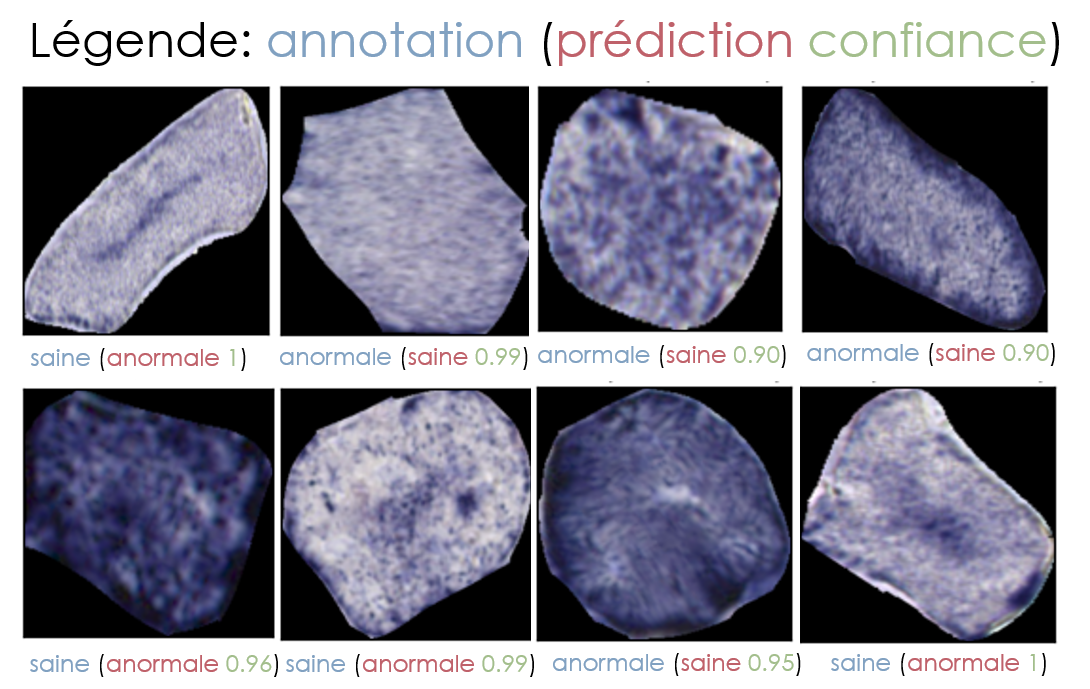
\includegraphics[width=1\textwidth]{figures/list_sdh_errors.png}
 \caption[Exemple de fibres ayant un label prédit contraire a l'annotation avec un haut niveau de confiance du modèle]{Exemple de fibres ayant un label prédit contraire a l'annotation avec un haut niveau de confiance du modèle}
 \label{fig:list_errors}
\end{figure}

\section{Déploiement de la plateforme}
Pour faciliter l'utilisation et la diffusion de \gls{myoquant} nous avons développé l'outil sous deux formes: un outil en ligne de commande et une version de démonstration en ligne.

\subsection{Outil en ligne de commande}
Sous sa forme d'outil en ligne de commande, \gls{myoquant} est téléchargeable comme bibliothèque Python disponible dans le répertoire officiel PyPI à l'adresse \href{https://pypi.org/project/myoquant/}{https://pypi.org/project/myoquant/}. La version en ligne de commande permet de traiter un grand nombre d'images et/ou des images de coupes complètes trop grandes pour être traitées via une interface en ligne. Ceci permet de traiter les images sur des serveurs de calcul équipés de \gls{gpu} afin d'accélérer le processus d'analyse et de sauvegarder l'ensemble des résultats.

\subsection{Version de démonstration en ligne}
\gls{myoquant} est aussi disponible sous forme d'interface de démonstration en ligne développée grâce à \textit{Streamlit}. Cette interface en ligne est utile pour faire des démonstrations de l'outil de façon visuelle notamment grâce aux différents graphiques d'explicabilité générés. Cette interface permet aussi de tester l'outil sur des images de petites tailles afin d'évaluer quels seraient les meilleurs paramètres pour obtenir une classification de qualité. \gls{myoquant}-Streamlit est disponible en ligne à l'adresse \href{https://lbgi.fr/MyoQuant/}{https://lbgi.fr/MyoQuant/} ainsi que sur \textit{HuggingFace Space} \href{https://huggingface.co/spaces/corentinm7/MyoQuant}{https://huggingface.co/spaces/corentinm7/MyoQuant}.

\section{Limites et perspectives de développement}
L'outil \gls{myoquant} permet de quantifier des marqueurs pathologiques dans trois des cinq colorations réalisées en routine pour le diagnostic des \gls{mc}. Pour l'instant, \gls{myoquant} n'inclut pas de méthode dédiée à l'analyse des coupes à la coloration \gls{tg} pour détecter les agrégats protéiques, ni de méthode pour la coloration NADH pouvant mettre en évidence la présence de \textit{cores}. Des modèles \gls{ia} suivant la même méthodologie que ce que nous avons développé pour la coloration \gls{sdh} devront être développé en conséquence. Il est aussi nécessaire pour certaine coloration d'élargir le champs des marqueurs pathologiques quantifiés. Par exemple pour la coloration \gls{he}, la taille des fibres et notamment la détection de fibres atrophiques est aussi évaluée en routine lors du diagnostic en plus de la position des noyaux.

De plus, \gls{myoquant} a majoritairement été développé à partir de données issues de biopsies musculaires de souris. Il serait intéressant de tester \gls{myoquant} sur un jeu de données de biopsies humaines quantifiées manuellement par un expert pour évaluer son niveau de performance sur des données humaines. En cas de performance satisfaisantes, il serait alors possible d'analyser de façon massive les données de patients afin d'établir de potentiels seuils pour chaque marqueurs pathologiques pour le diagnostic automatique de \gls{mc}.

 Enfin, sur un plan technique, il serait intéressant de développer une interface en ligne pour \gls{myoquant} liée à des \gls{gpu} pour le traitement de coupes complètes en un temps raisonnable sans avoir à utiliser la ligne de commande, qui est un frein majeur pour un public non expérimenté en programmation, ce qui est typiquement le cas lors du diagnostic.